% Digital Logic Lab 1 Report
% Created: 2020-01-15, Jane Ross

%==========================================================
%=========== Document Setup  ==============================

% Formatting defined by class file
\documentclass[11pt]{article}

% ---- Document formatting ----
\usepackage[margin=1in]{geometry}	% Narrower margins
\usepackage{booktabs}				% Nice formatting of tables
\usepackage{graphicx}				% Ability to include graphics

%\setlength\parindent{0pt}	% Do not indent first line of paragraphs 
\usepackage[parfill]{parskip}		% Line space b/w paragraphs
%	parfill option prevents last line of pgrph from being fully justified

% Parskip package adds too much space around titles, fix with this
\RequirePackage{titlesec}
\titlespacing\section{0pt}{8pt plus 4pt minus 2pt}{3pt plus 2pt minus 2pt}
\titlespacing\subsection{0pt}{4pt plus 4pt minus 2pt}{-2pt plus 2pt minus 2pt}
\titlespacing\subsubsection{0pt}{2pt plus 4pt minus 2pt}{-6pt plus 2pt minus 2pt}

% ---- Hyperlinks ----
\usepackage[colorlinks=true,urlcolor=blue]{hyperref}	% For URL's. Automatically links internal references.

% ---- Code listings ----
\usepackage{listings} 					% Nice code layout and inclusion
\usepackage[usenames,dvipsnames]{xcolor}	% Colors (needs to be defined before using colors)

% Define custom colors for listings
\definecolor{listinggray}{gray}{0.98}		% Listings background color
\definecolor{rulegray}{gray}{0.7}			% Listings rule/frame color

% Style for Verilog
\lstdefinestyle{Verilog}{
	language=Verilog,					% Verilog
	backgroundcolor=\color{listinggray},	% light gray background
	rulecolor=\color{blue}, 			% blue frame lines
	frame=tb,							% lines above & below
	linewidth=\columnwidth, 			% set line width
	basicstyle=\small\ttfamily,	% basic font style that is used for the code	
	breaklines=true, 					% allow breaking across columns/pages
	tabsize=3,							% set tab size
	commentstyle=\color{gray},	% comments in italic 
	stringstyle=\upshape,				% strings are printed in normal font
	showspaces=false,					% don't underscore spaces
}

% How to use: \Verilog[listing_options]{file}
\newcommand{\Verilog}[2][]{%
	\lstinputlisting[style=Verilog,#1]{#2}
}




%======================================================
%=========== Body  ====================================
\begin{document}

\title{ELC 2137 Lab 1: Git and LaTex Intro}
\author{Jane Ross}

\maketitle


\section*{Summary}

The objective of this lab is to describe the basic Git process, use GitHub Desktop to synchronize locaol and remote files ina repository. Also describe the purpose of LaTeX and create a lab report in LaTeX that includes images, codes, lists,tables and section headings. 


\section*{Q\&A}

\begin{enumerate}
	\item 
	My GitHub user name is jane-ross1.
	\item
	A bulleted list is configured using an itemized enviroment.
	\item 
		$ y(t) = 1/2 e^t $
	\item 
	A shortcut to compile is F6 on the windows computer.
	
\end{enumerate}


\section*{Results}



\begin{figure}[ht]\centering
	
	\begin{tabular}{c|c|c}
		\toprule
		Binary & Hex & Decimal \\
		\midrule
		0000 & 0 & 0 \\
		0010 & 2 & 2 \\
		0100 & 4 & 4 \\
		0110 & 6 & 6 \\
		1000 & 8 & 8 \\
		1010 & A & 10 \\
		\bottomrule
	\end{tabular}

	\centering
	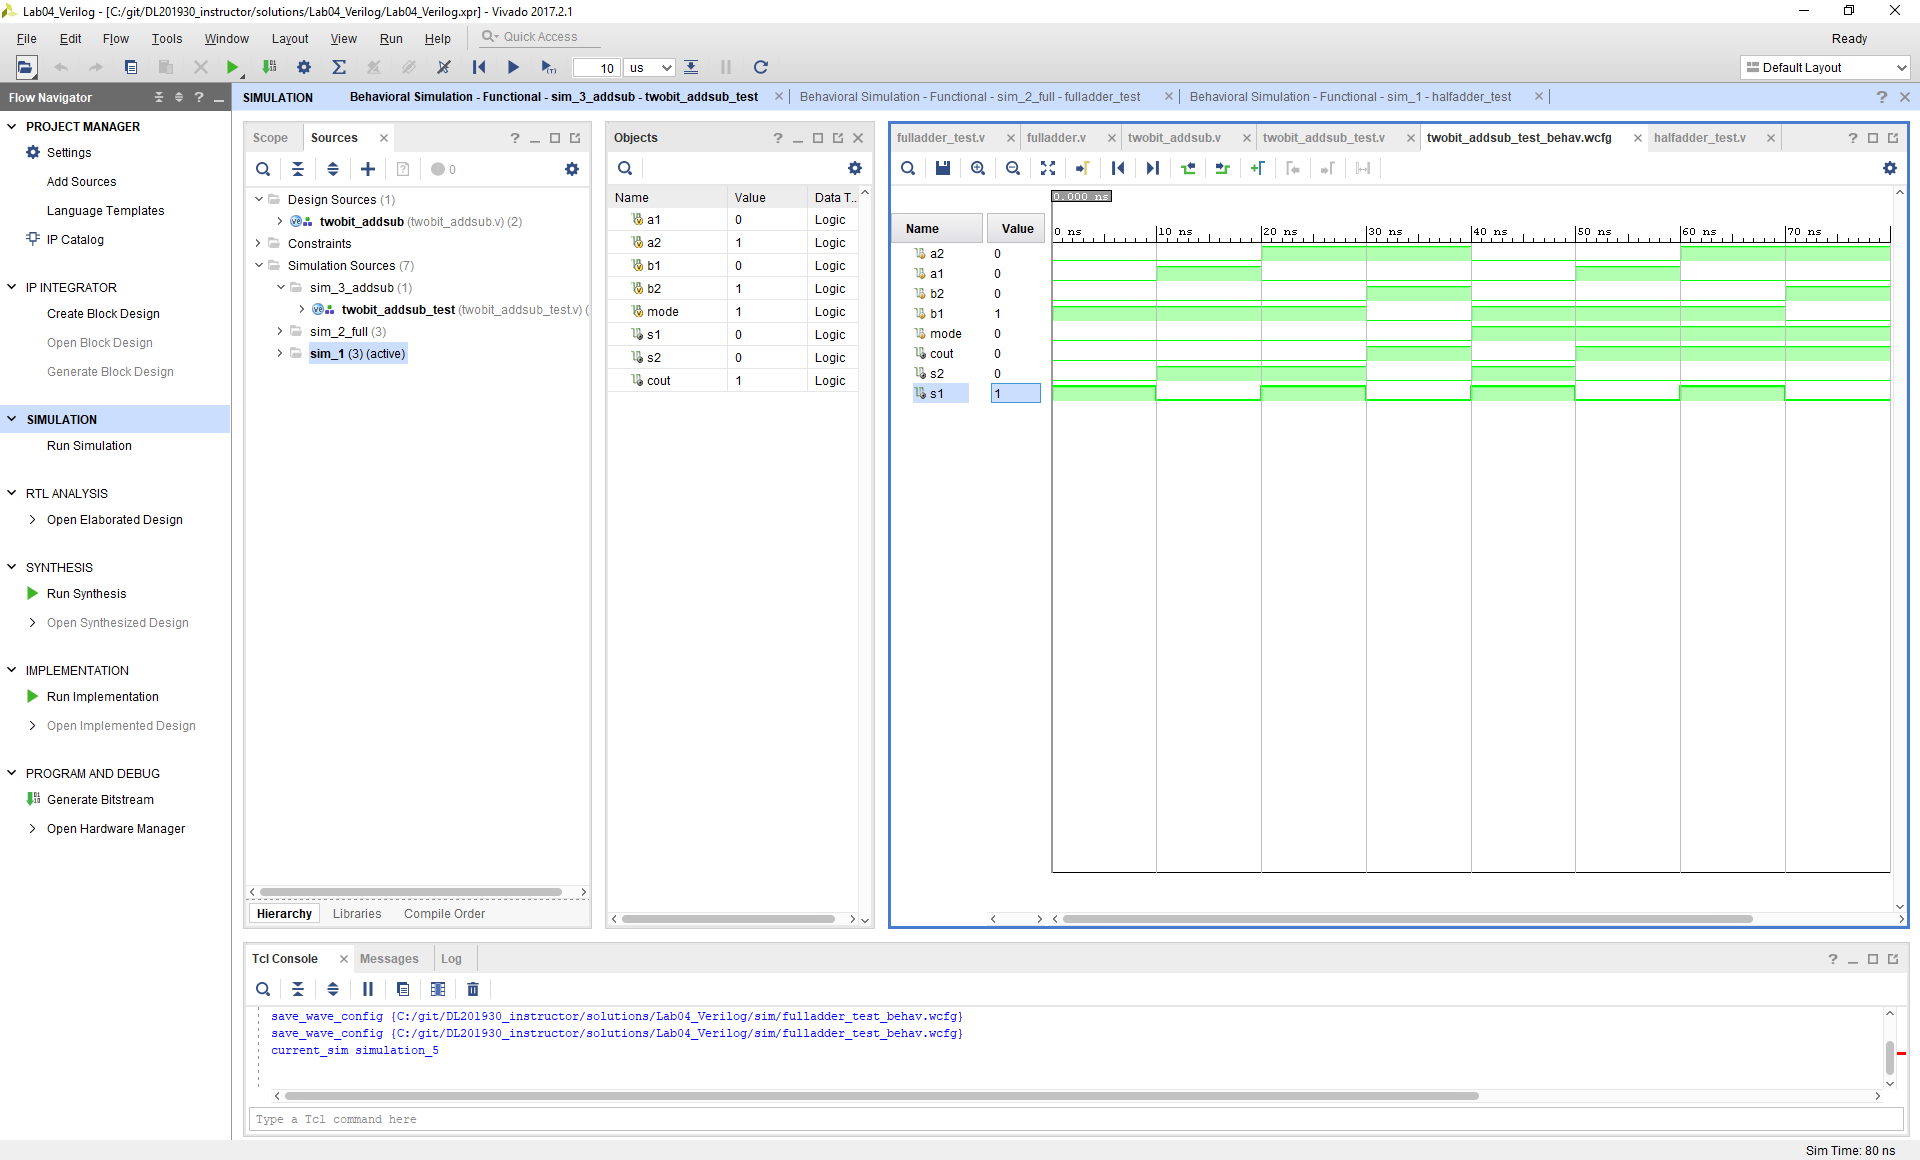
\includegraphics[scale = 0.70,trim={18cm 15cm 0 4cm},clip]{lab1_example_screenshot}

	\caption{Table and simulation waveform to reproduce}
	\label{fig:lab1examplescreenshot}

\end{figure}

	

	
\begin{figure}
	\centering
	\includegraphics[width=0.7\linewidth]{"Screenshot of history"}
	\caption{Screenshot}
	\label{fig:screenshot-of-history}
\end{figure}




\section*{Code}

This is the code example below.
\begin{lstlisting}[style=Verilog,
caption=Direct Verilog code example,
label=code:ex 
]
module example
#(parameter BITS=4)
(
input [BITS-1:0] in0, in1,
input sel,
output [BITS-1:0] out
);

// Choose in1 or in0
out = sel ? in1: in0; 
endmodule
\end{lstlisting}
\end{document}
